% Editable master. Rebuild the PDF and theme-aware SVG with: python3 build.py
\documentclass[10pt,tikz,border=10pt]{standalone}
\usepackage[T1]{fontenc}
\usepackage{helvet}
\usepackage{amssymb}
\renewcommand{\familydefault}{\sfdefault}
\usetikzlibrary{arrows.meta,calc}
\definecolor{ink}{HTML}{1E293B}
\definecolor{muted}{HTML}{536277}
\definecolor{boundary}{HTML}{94A3B8}
\definecolor{volume}{HTML}{F3F6FA}
\definecolor{inflow}{HTML}{2463A8}
\definecolor{outflow}{HTML}{137B69}
\ifdefined\darkmode
  \definecolor{ink}{HTML}{E6EDF5}
  \definecolor{muted}{HTML}{B4C1D2}
  \definecolor{boundary}{HTML}{8294AD}
  \definecolor{volume}{HTML}{202D3D}
  \definecolor{inflow}{HTML}{7DB9F2}
  \definecolor{outflow}{HTML}{79CFBA}
  \definecolor{canvas}{HTML}{121923}
  \pagecolor{canvas}
\fi
\begin{document}
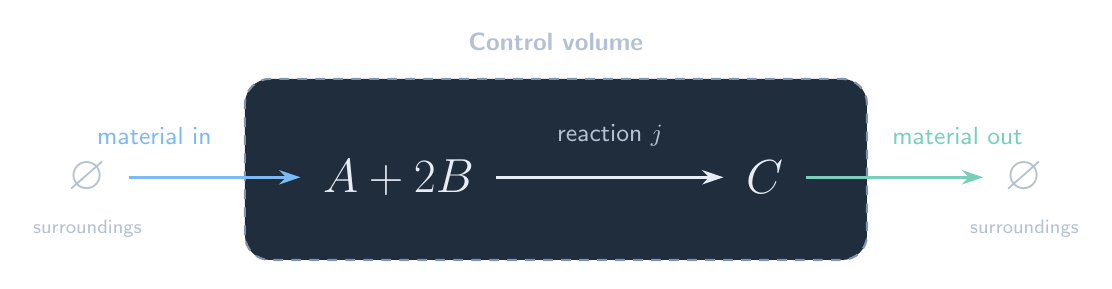
\begin{tikzpicture}[x=1cm,y=1cm,
  every node/.style={text=ink,font=\sffamily,inner sep=2pt},
  flow/.style={-{Stealth[length=2.7mm,width=1.8mm]},line width=1.2pt},
  species/.style={font=\LARGE,inner sep=0pt},
  note/.style={font=\sffamily\small,text=muted},
  reservoir note/.style={font=\sffamily\scriptsize,text=muted}]

% The two external reservoirs remain outside the modeled control volume.
\path[fill=volume,draw=boundary,line width=.75pt,
  dash pattern=on 3.5pt off 3pt,rounded corners=9pt]
  (2.45,-1.05) rectangle (10.35,1.25);
\node[font=\sffamily\bfseries\small,text=muted] at (6.4,1.72)
  {Control volume};

\node[species,text=muted] (source) at (.45,0) {$\varnothing$};
\node[species,text=muted] (sink) at (12.35,0) {$\varnothing$};
\node[reservoir note] at (.45,-.65) {surroundings};
\node[reservoir note] at (12.35,-.65) {surroundings};

\node[species] (reactants) at (4.40,0) {$A+2B$};
\node[species] (product) at (9.05,0) {$C$};
% Equal clearances keep arrowheads separate from the mathematical glyphs.
\draw[flow,draw=inflow] ($(source.east)+(.28,0)$)--($(reactants.west)-(.28,0)$);
\draw[flow,draw=ink] ($(reactants.east)+(.28,0)$)--($(product.west)-(.28,0)$)
  node[midway,yshift=.53cm,note] {reaction $j$};
\draw[flow,draw=outflow] ($(product.east)+(.28,0)$)--($(sink.west)-(.28,0)$);

\node[note,text=inflow] at (1.3,.53) {material in};
\node[note,text=outflow] at (11.5,.53) {material out};
\end{tikzpicture}
\end{document}
